\documentclass[11pt,a4paper]{article}
\usepackage[utf8]{inputenc}
\usepackage[spanish,es-tabla,es-noquoting]{babel}
\usepackage[margin=2.5cm]{geometry}
\usepackage{graphicx}
\usepackage{amsmath,amssymb}
\usepackage{booktabs}
\usepackage{xcolor}
\usepackage{hyperref}
\usepackage{tikz}
\usetikzlibrary{shapes.geometric, arrows, positioning, fit, calc}
\usepackage{fancyhdr}
\usepackage{caption}
\usepackage{subcaption}
\usepackage{enumitem}

% Configuración de colores corporativos
\definecolor{primaryblue}{RGB}{24, 76, 120}
\definecolor{accentgreen}{RGB}{39, 174, 96}
\definecolor{accentred}{RGB}{192, 57, 43}
\definecolor{accentamber}{RGB}{211, 84, 0}
\definecolor{cardbg}{RGB}{248, 250, 252}
\definecolor{bordercolor}{RGB}{226, 232, 240}

% Definición de caja personalizada nativa con lrbox (sin dependencias externas)
\setlength{\fboxsep}{10pt}
\setlength{\fboxrule}{1pt}
\newsavebox{\customboxstorage}
\newenvironment{custombox}[2][primaryblue]{%
    \def\customboxcolor{#1}%
    \begin{lrbox}{\customboxstorage}%
    \begin{minipage}{0.92\textwidth}%
    \if\relax\detokenize{#2}\relax\else\textbf{\color{#1}#2}\par\vspace{6pt}\fi
}{%
    \end{minipage}%
    \end{lrbox}%
    \begin{center}%
    \fcolorbox{\customboxcolor}{cardbg}{\usebox{\customboxstorage}}%
    \end{center}%
}

% Configuración de hipervínculos
\hypersetup{
    colorlinks=true,
    linkcolor=primaryblue,
    citecolor=accentgreen,
    urlcolor=primaryblue
}

% Encabezados y pie de página
\pagestyle{fancy}
\fancyhf{}
\rhead{\color{gray}\small QuickDelivery Sim --- Guía Maestra Exhaustiva}
\lhead{\color{gray}\small Modelos y Simulación}
\rfoot{\thepage}

% Estilos de diagramas TikZ
\tikzstyle{startstop} = [rectangle, rounded corners=6pt, minimum width=2.8cm, minimum height=0.9cm, text centered, draw=primaryblue, fill=primaryblue!10, font=\small\bfseries, align=center]
\tikzstyle{process} = [rectangle, rounded corners=3pt, minimum width=2.8cm, minimum height=0.9cm, text centered, draw=primaryblue!80, fill=white, font=\small, align=center]
\tikzstyle{decision} = [diamond, aspect=1.8, minimum width=2.5cm, minimum height=0.8cm, text centered, draw=accentamber!90, fill=accentamber!15, font=\footnotesize\bfseries, align=center]
\tikzstyle{sublink} = [rectangle, rounded corners=8pt, minimum width=2.6cm, minimum height=0.8cm, text centered, draw=primaryblue, fill=primaryblue!85, text=white, font=\small\bfseries, align=center]
\tikzstyle{cancelbox} = [rectangle, rounded corners=3pt, minimum width=2.6cm, minimum height=0.8cm, text centered, draw=accentred!90, fill=accentred!15, font=\footnotesize\bfseries, align=center]
\tikzstyle{arrow} = [thick,->,>=stealth,color=primaryblue]
\tikzstyle{dasharrow} = [thick,dashed,->,>=stealth,color=accentred]
\tikzstyle{classbox} = [rectangle, draw=primaryblue, fill=cardbg, rounded corners=4pt, inner sep=6pt, text width=3.4cm, font=\small]

\begin{document}

% ==============================================================================
% PORTADA
% ==============================================================================
\begin{titlepage}
    \centering
    \vspace*{1cm}
    
    {\Huge \textbf{\color{primaryblue} QuickDelivery Sim}}\\[0.5cm]
    {\LARGE \textbf{Gemelo Digital y Optimización Inteligente de Entregas a Domicilio en Tiempo Real}}\\[1cm]
    
    {\large \textbf{Documento Maestro Exhaustivo y Guía Explicativa del Proyecto}}\\[0.3cm]
    {\normalsize Explicación profunda de extremo a extremo en lenguaje común y accesible}\\[1.5cm]
    
    \begin{custombox}[primaryblue]{}
        \centering
        \textbf{Institución Universitaria Pascual Bravo}\\[0.2cm]
        Facultad de Ingeniería --- Curso de Modelos y Simulación (2026-2)\\[0.2cm]
        \textbf{Equipo Desarrollador (Grupo 2):}\\[0.15cm]
        \begin{tabular}{ll}
            \textbf{Sebastian Echeverri} & Modelado de Simulación y Reglas Operativas \\
            \textbf{Juan Manuel Jaramillo} & Arquitectura de Software, API y Telemetría \\
            \textbf{Emmanuel Mora} & Análisis Estadístico y Validación Analítica \\
        \end{tabular}
    \end{custombox}
    
    \vfill
    
    \begin{custombox}[bordercolor]{}
        \small
        \textbf{Propósito de este documento:} Servir como memoria técnica integral y puente pedagógico para que cualquier integrante del equipo, docente o evaluador externo comprenda qué problema se resuelve, cómo se implementó la arquitectura de software real con su panel de control interactivo, cómo funciona el simulador y qué decisiones operativas respaldan los datos.
    \end{custombox}
    
    \vspace{0.8cm}
    {\small Medellín, Colombia --- Noviembre de 2026}
\end{titlepage}

\tableofcontents
\newpage

% ==============================================================================
% SECCIÓN 1: INTRODUCCIÓN Y CONTEXTO
% ==============================================================================
\section{Introducción y Contexto de la Empresa}

\subsection{El Negocio de las Entregas Rápidas en la Ciudad}
Imagine una ciudad viva y dinámica como Medellín o Bogotá. En cualquier momento del día, miles de personas sienten hambre, abren su teléfono móvil y solicitan comida a través de una aplicación. En menos de cuarenta minutos, esperan recibir una pizza crujiente o una hamburguesa recién salida de la parrilla en la puerta de su hogar.

Detrás de este simple clic en el teléfono, existe un engranaje operativo inmenso y complejo que involucra a tres protagonistas clave:
\begin{enumerate}[label=\textbf{\arabic*.}]
    \item \textbf{El Cliente Comprador:} Es la persona que realiza el pedido. Posee un límite de paciencia natural: si el restaurante o el repartidor tardan más de lo razonable, el cliente se impacienta, se desanima y puede cancelar el pedido, generando una pérdida económica total para la plataforma.
    \item \textbf{Los Restaurantes Aliados:} Son locales comerciales con cocinas de tamaño físico limitado. Cada local tiene un número fijo de fogones o estaciones de cocina. Si todos los fogones están ocupados con hamburguesas o pizzas, cualquier nuevo pedido debe esperar en una fila virtual de cocina. La comida toma un tiempo físico en cocinarse y, al finalizar, se coloca en un mostrador de despacho esperando a quien la transporte.
    \item \textbf{Los Repartidores Autónomos (Flota Abierta):} Son personas en motocicleta o bicicleta que se conectan libremente a la aplicación cuando desean trabajar. La plataforma no les paga un salario por estar sentados esperando; ellos ganan dinero por pedido entregado. Se desplazan por las calles esquivando tráfico, y dependen de la batería de su teléfono celular para recibir instrucciones de la aplicación.
\end{enumerate}

\subsection{El Gran Desafío: El Choque de Dos Tiempos Distintos}
El problema más grave que enfrentan las plataformas modernas de entrega se resume en una frase cotidiana: \textbf{la desincronización entre la cocina y la calle}.

Cocinar un plato caliente toma un tiempo variable (usualmente entre 15 y 25 minutos). Por otro lado, viajar en motocicleta desde cualquier punto de la ciudad hasta el restaurante toma otro tiempo totalmente distinto (usualmente entre 5 y 10 minutos).

¿Qué ocurre si la plataforma avisa al repartidor en el instante exacto en que el cliente pulsa ``Comprar''?
El repartidor enciende su moto, llega al restaurante a toda velocidad en 6 minutos, entra apurado al local\dots{} ¡y descubre que la comida apenas lleva 6 minutos sobre el fuego y aún le faltan 15 minutos de cocción!
El repartidor queda atrapado en el local esperando de brazos cruzados, perdiendo tiempo valioso en el que podría estar entregando otros pedidos.

¿Y qué ocurre si la plataforma espera hasta que la comida esté completamente cocinada en el mostrador para recién buscar un repartidor?
La comida queda reposando en una bolsa de papel en el mostrador. Mientras la plataforma encuentra a un conductor libre y este viaja hasta el restaurante, transcurren 15 o 20 minutos. Cuando el repartidor finalmente llega, la comida ya perdió su temperatura óptima, las papas fritas perdieron su textura crujiente y el cliente recibe un producto de mala calidad.

El propósito central de este proyecto, denominado \textbf{QuickDelivery Sim}, es crear un cerebro informático capaz de predecir ambos tiempos y coordinar con precisión milimétrica la cocina y el despacho, logrando que el repartidor llegue al restaurante casi al mismo tiempo en que la comida sale del fogón.

% ==============================================================================
% SECCIÓN 2: PLANTEAMIENTO DEL PROBLEMA
% ==============================================================================
\section{Planteamiento del Problema y Limitaciones del Mundo Real}

\subsection{La Política Tradicional y sus Errores (Asignación Voraz Inmediata)}
En los sistemas de primera generación se utilizaba una estrategia llamada \textbf{Asignación Voraz Inmediata}. Su regla era muy ingenua:
\begin{quote}
\textit{``Apenas entra una orden, busca inmediatamente al repartidor más cercano y asígnale el pedido de inmediato.''}
\end{quote}

Esta estrategia genera tres consecuencias desastrosas para el negocio:
\begin{itemize}[leftmargin=*]
    \item \textbf{Ociosidad excesiva del conductor:} Como se demostró en los datos reales del proyecto, el repartidor pasaba en promedio \textbf{casi 11 minutos esperando sentado en el restaurante} por cada pedido. En horas pico, esta espera alcanzaba los 16 minutos.
    \item \textbf{Agotamiento artificial de la flota:} Si 30 repartidores están retenidos esperando comida cruda dentro de los restaurantes, la plataforma se queda sin conductores disponibles en las calles.
    \item \textbf{Efecto dominó de enfriamiento:} Paradójicamente, cuando otro restaurante terminaba de cocinar un pedido listo para entregar, no había conductores libres en la calle porque todos estaban atrapados esperando en otros locales. La comida lista terminaba enfriándose en el mostrador más de 12 minutos.
\end{itemize}

\subsection{Las Tres Restricciones Físicas Duras del Sistema Real}
Para que este estudio tuviera validez en el mundo real y no fuera un simple ejercicio académico teórico, se incorporaron tres límites físicos inquebrantables:
\begin{enumerate}[label=\textbf{\alph*.}]
    \item \textbf{Capacidad de Fogones en Cocina (Tope Físico de 47 Fogones):} La red de 10 restaurantes suma un total de 47 fogones instalados. Aunque entren 200 pedidos en una hora de almuerzo, las cocinas físicamente no pueden preparar más de 2.5 pedidos por minuto simultáneamente.
    \item \textbf{Capacidad del Servidor de Base de Datos (Tope de 30 Conexiones):} El sistema informático central (PostgreSQL) cuenta con un límite estricto de 30 conexiones simultáneas. Si cientos de repartidores envían su posición GPS cada dos segundos, el servidor se satura y la aplicación se congela.
    \item \textbf{Autonomía Energética del Móvil (Corte Preventivo al 15\% de Batería):} La aplicación de despacho consume batería por el uso constante del GPS y la pantalla. Si el nivel de carga de un repartidor cae por debajo del 15\%, la aplicación no le asigna viajes largos para evitar que el teléfono se apague en mitad de una entrega.
\end{enumerate}

% ==============================================================================
% SECCIÓN 3: ARQUITECTURA DEL SISTEMA REAL Y API
% ==============================================================================
\section{Arquitectura del Sistema Real y la API de Servicios}

\subsection{Construcción Modular y Contenerizada}
El sistema no es únicamente una simulación matemática: cuenta con un prototipo de software real desarrollado en lenguaje Python con el framework \textbf{FastAPI} y respaldado por una base de datos relacional robusta. Todo el entorno se encuentra empaquetado mediante contenedores \textbf{Docker Compose}, lo que garantiza que cualquier ingeniero pueda ejecutarlo en Windows, Linux o Mac con un único comando.

\begin{figure}[htbp]
\centering
\resizebox{\textwidth}{!}{%
\begin{tikzpicture}[auto]
    % --- Fila Superior: Actores y Canales Externos ---
    \node [classbox, text width=3.7cm, minimum height=2.6cm] (cliente) at (0, 0) {
        \textbf{\color{primaryblue} 1. Cliente (App / Web)}\\[0.1cm]
        \scriptsize $\bullet$ Crea comanda con $(x,y)$\\
        $\bullet$ Monitoreo en tiempo real\\
        $\bullet$ Abandono por impaciencia
    };
    
    \node [classbox, text width=3.7cm, minimum height=2.6cm] (kds) at (4.3, 0) {
        \textbf{\color{primaryblue} 2. Restaurante (KDS)}\\[0.1cm]
        \scriptsize $\bullet$ 10 restaurantes ($k_r \in [3,6]$)\\
        $\bullet$ 47 fogones en total\\
        $\bullet$ Notificación plato listo
    };
    
    \node [classbox, text width=3.7cm, minimum height=2.6cm] (repartidor) at (8.6, 0) {
        \textbf{\color{primaryblue} 3. Repartidor (GPS)}\\[0.1cm]
        \scriptsize $\bullet$ Ventana de oferta de 45 s\\
        $\bullet$ Telemetría y cinemática\\
        $\bullet$ Control batería $\ge 15\%$
    };
    
    \node [classbox, text width=3.7cm, minimum height=2.6cm, draw=accentgreen] (dash_actor) at (12.9, 0) {
        \textbf{\color{accentgreen} 4. Dashboard (NiceGUI)}\\[0.1cm]
        \scriptsize $\bullet$ Plano Cartesiano interactivo\\
        $\bullet$ Simulación sin consola\\
        $\bullet$ Métricas y hardware
    };
    
    % --- Fila Media: Núcleo FastAPI ---
    \node [rectangle, draw=primaryblue, fill=primaryblue!5, rounded corners=6pt, inner sep=12pt, text width=16.0cm] (api) at (6.45, -3.8) {
        \centering
        \textbf{\color{primaryblue}\large Cerebro Central: API REST FastAPI (Uvicorn :8000)}\\[0.25cm]
        \begin{minipage}{0.31\textwidth}
            \textbf{\color{primaryblue}Gestor de Órdenes}\\
            \scriptsize $\bullet$ Ingestión de pedidos\\
            $\bullet$ Control de fogones (FIFO)\\
            $\bullet$ Estimación de $\text{ETA}_{\text{listo}}$
        \end{minipage}
        \hfill
        \begin{minipage}{0.33\textwidth}
            \textbf{\color{primaryblue}Motor de Despacho}\\
            \scriptsize $\bullet$ Patrón Strategy\\
            $\bullet$ Sincronización predictiva\\
            $\bullet$ Escalamiento en 2 fases
        \end{minipage}
        \hfill
        \begin{minipage}{0.31\textwidth}
            \textbf{\color{primaryblue}Telemetría y Control}\\
            \scriptsize $\bullet$ Middleware latencia HTTP\\
            $\bullet$ Monitoreo CPU / RAM\\
            $\bullet$ QueuePool PostgreSQL
        \end{minipage}
    };
    
    % --- Fila Inferior: Persistencia y Almacén ---
    \node [classbox, text width=7.4cm, minimum height=2.5cm] (db) at (2.4, -7.2) {
        \textbf{\color{primaryblue} Base de Datos Relacional (PostgreSQL 15)}\\[0.1cm]
        \scriptsize $\bullet$ Tablas: \texttt{orders}, \texttt{restaurants}, \texttt{couriers}, \texttt{tracking}\\
        $\bullet$ \textbf{Cota dura C6:} Pool limitado a 30 conexiones (\texttt{QueuePool})\\
        $\bullet$ Transacciones ACID con bloqueo de fila concurrente seguro
    };
    
    \node [classbox, text width=7.4cm, minimum height=2.5cm] (telemetry_file) at (10.5, -7.2) {
        \textbf{\color{accentamber} Almacén de Telemetría y Métricas}\\[0.1cm]
        \scriptsize $\bullet$ Archivo de telemetría: \texttt{datos/telemetry\_log.csv} ($n=710$)\\
        $\bullet$ Resultados de simulación: \texttt{datos/simulation\_results.json}\\
        $\bullet$ Barrido de sensibilidad: \texttt{datos/sensibilidad\_buffer\_results.json}
    };
    
    % --- Flechas Verticales Superiores (Actores -> API) ---
    \draw [arrow] (cliente.south) -- (api.north -| cliente.south) node [midway, right=1pt] {\scriptsize HTTPS};
    \draw [arrow] (kds.south) -- (api.north -| kds.south) node [midway, right=1pt] {\scriptsize Listo};
    \draw [arrow] (repartidor.south) -- (api.north -| repartidor.south) node [midway, right=1pt] {\scriptsize GPS};
    \draw [arrow] (dash_actor.south) -- (api.north -| dash_actor.south) node [midway, right=1pt] {\scriptsize Web};
    
    % --- Flechas Verticales Inferiores (API <-> DB / Archivos) ---
    \draw [thick,<->,>=stealth,color=primaryblue] (api.south -| db.north) -- (db.north) node [midway, right=2pt] {\scriptsize SQLAlchemy};
    \draw [arrow] (api.south -| telemetry_file.north) -- (telemetry_file.north) node [midway, right=2pt] {\scriptsize Exportación};
\end{tikzpicture}%
}
\caption{Diagrama de Arquitectura Multicontenedor del Sistema Real, Servicios Núcleo y Flujos de Comunicación.}
\label{fig:arquitectura_sistema}
\end{figure}

\subsection{Modelo de Datos y Clases Principales}
En lugar de manejar tablas confusas, el sistema organiza la información en cuatro entidades claras:
\begin{itemize}[leftmargin=*]
    \item \textbf{Pedido (\texttt{OrderModel}):} Contiene el identificador único, el cliente solicitante, el restaurante asignado, las coordenadas exactas de entrega, el estado actual de la comanda (por ejemplo: \textit{En Cola de Cocina}, \textit{En Preparación}, \textit{Listo en Mostrador}, \textit{En Tránsito} o \textit{Entregado}) y el cálculo del tiempo estimado de preparación.
    \item \textbf{Restaurante (\texttt{RestaurantModel}):} Representa a cada uno de los 10 locales de la ciudad, guardando su posición geográfica fija y su límite de fogones físicos.
    \item \textbf{Repartidor (\texttt{CourierModel}):} Modela al conductor con su nombre, posición actual en la ciudad, porcentaje de batería remanente y bandera de disponibilidad.
    \item \textbf{Registro de Ubicación (\texttt{TrackingRecordModel}):} Guarda el histórico de telemetría GPS para auditoría y medición de latencias.
\end{itemize}

% ==============================================================================
% SECCIÓN 4: EL DASHBOARD INTERACTIVO
% ==============================================================================
\section{El Centro de Operaciones Interactivo (Dashboard Web)}

\subsection{¿Por qué se creó este Panel Visual?}
Para interactuar con una API tradicional, un ingeniero suele verse obligado a utilizar herramientas complejas como Postman o redactar comandos manuales de consola (\texttt{curl}). Esto resulta lento, propenso a errores y poco comprensible para personas de negocios.

Por ello, se implementó un \textbf{Centro de Operaciones en Tiempo Real} utilizando la librería \textbf{NiceGUI}. Este panel permite que cualquier usuario manipule y observe todo el ecosistema de entrega de forma completamente visual, automatizada y sin necesidad de escribir una sola línea de código.

\subsection{Explicación Profunda de la Pantalla de Operaciones (Plano 2D)}
La primera vista del panel está dedicada al control geográfico de la ciudad y al ciclo de vida de los pedidos:

\begin{figure}[htbp]
    \centering
    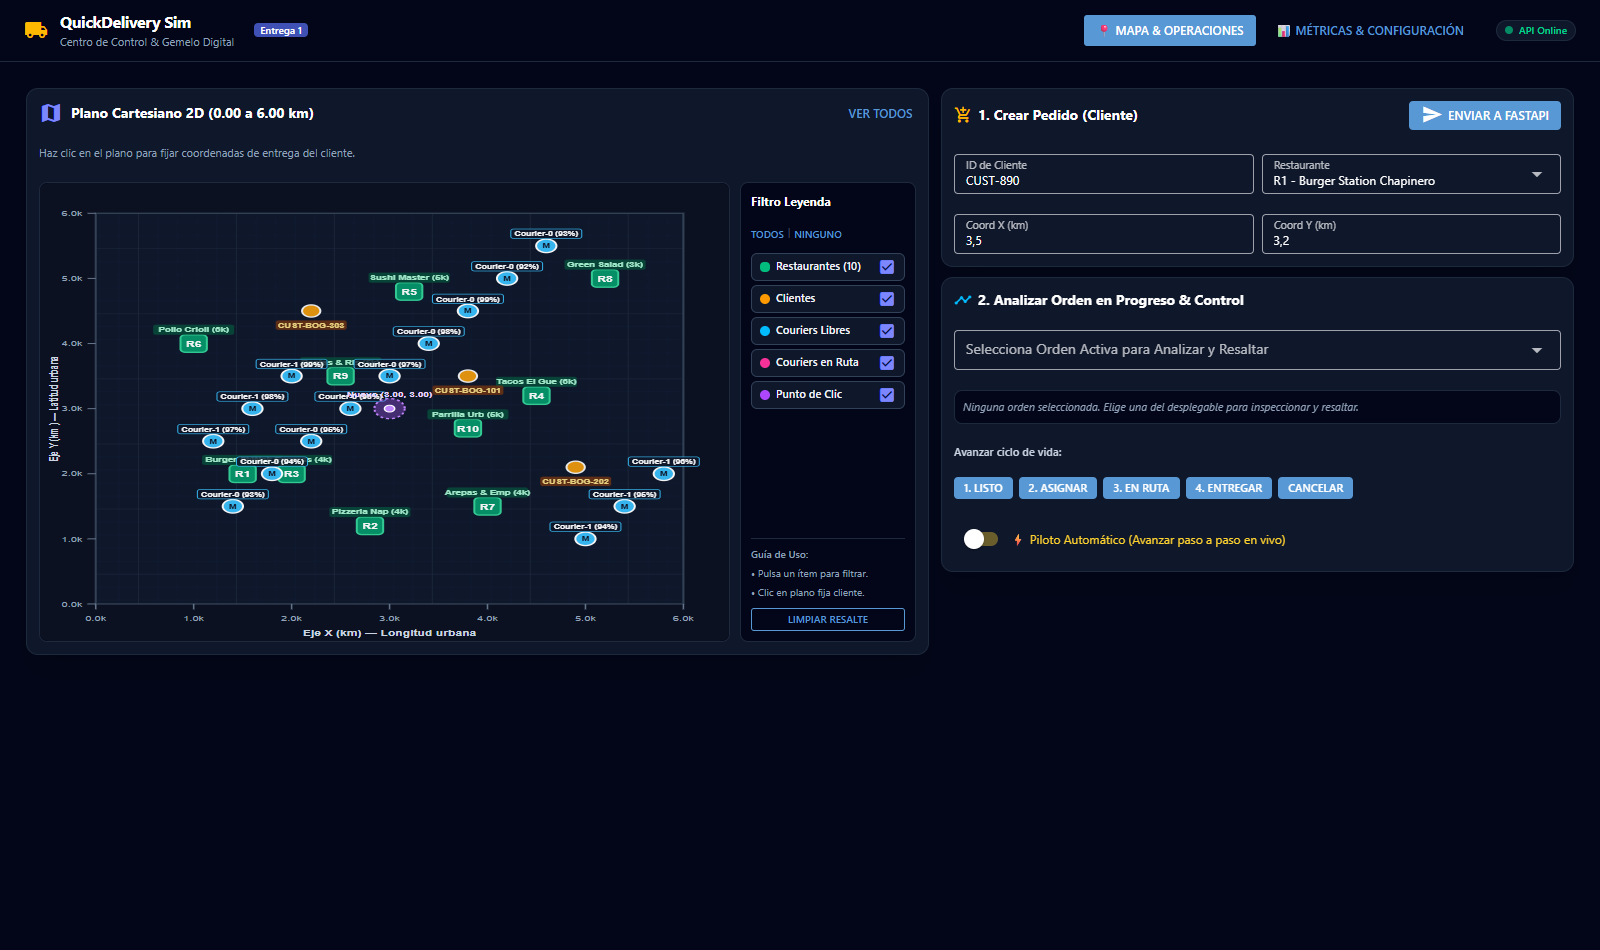
\includegraphics[width=0.95\textwidth]{figuras/fig_05_dashboard_operaciones.png}
    \caption{Vista de Operaciones en Tiempo Real: Plano Cartesiano 2D, Leyendas Dinámicas y Controles de Despacho.}
    \label{fig:dash_operaciones}
\end{figure}

Al observar la \textbf{Figura~\ref{fig:dash_operaciones}}, se aprecian los siguientes componentes diseñados para máxima facilidad de uso:
\begin{itemize}[leftmargin=*]
    \item \textbf{Plano Cartesiano de la Ciudad (Izquierda):} Muestra una cuadrícula exacta de $6 \times 6\text{ kilómetros}$. En ella se ubican visualmente los 10 restaurantes con iconos cuadrados esmeralda, los repartidores disponibles en color celeste, los repartidores que van en camino en color rosado y las entregas a clientes en color ámbar.
    \item \textbf{Fijación de Coordenadas por Clic:} Si el usuario desea crear un pedido para un cliente, no necesita escribir números de latitud ni longitud: simplemente hace clic sobre cualquier punto del mapa y el sistema traduce el píxel en coordenadas de kilómetros exactas.
    \item \textbf{Panel Superior de Creación de Pedidos (Derecha Arriba):} Permite seleccionar el restaurante emisor, ingresar el identificador del cliente y pulsar el botón morado \textbf{``Enviar a FastAPI''}. En ese instante, la API registra el pedido y evalúa de inmediato si ingresa directo al fuego o espera en cola.
    \item \textbf{Panel de Inspección y Ciclo de Vida (Derecha Abajo):} El usuario puede seleccionar cualquier orden activa y avanzar manualmente su estado mediante botones secuenciales:
    \begin{center}
        \colorbox{cardbg}{\textbf{1. Marcar Listo}} $\longrightarrow$ 
        \colorbox{cardbg}{\textbf{2. Asignar Courier}} $\longrightarrow$ 
        \colorbox{cardbg}{\textbf{3. En Ruta}} $\longrightarrow$ 
        \colorbox{cardbg}{\textbf{4. Entregar}}
    \end{center}
    \item \textbf{Interruptor de Piloto Automático:} Al encender este botón de color amarillo, el sistema se encarga de avanzar la orden de manera autónoma segundo a segundo, simulando en vivo el paso del tiempo real.
\end{itemize}

\subsection{Explicación Profunda de la Pantalla de Métricas y Telemetría}
La segunda vista del panel se enfoca en la salud técnica y operativa del negocio:

\begin{figure}[htbp]
    \centering
    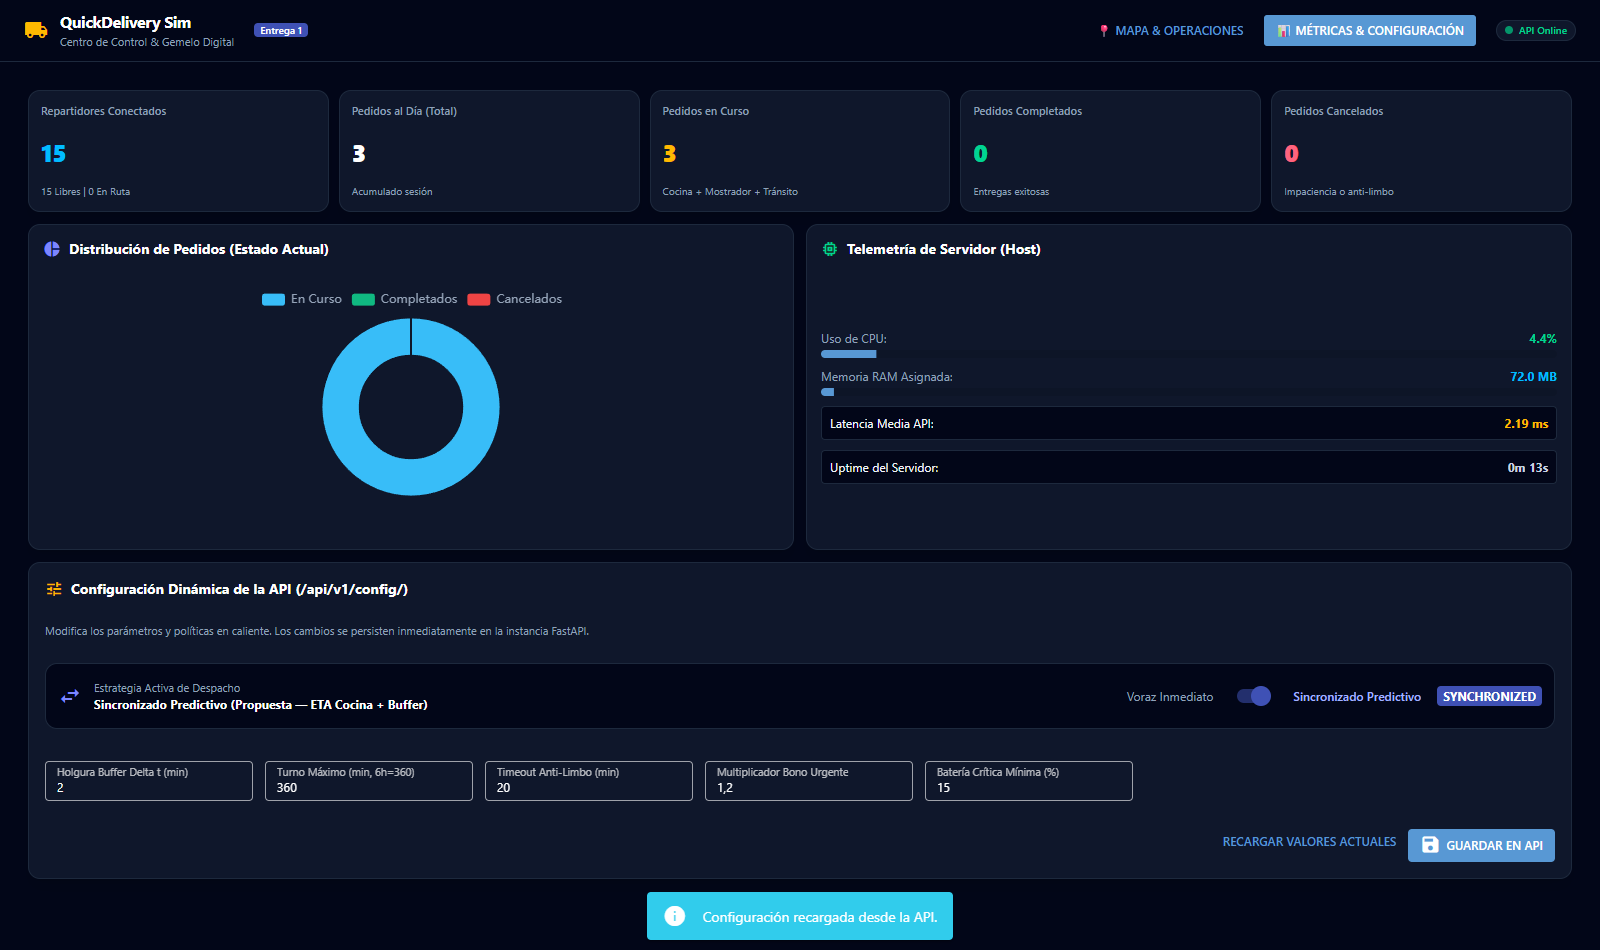
\includegraphics[width=0.95\textwidth]{figuras/fig_06_dashboard_metricas.png}
    \caption{Vista de Métricas y Telemetría: Tarjetas de Rendimiento, Distribución de Órdenes y Salud de Infraestructura.}
    \label{fig:dash_metricas}
\end{figure}

Como se aprecia en la \textbf{Figura~\ref{fig:dash_metricas}}, esta pantalla consolida los indicadores indispensables para la toma de decisiones:
\begin{itemize}[leftmargin=*]
    \item \textbf{Tarjetas Superiores de Resumen:} Informan en grandes números cuántos repartidores están conectados en este instante, cuántos pedidos se han completado con éxito hoy, cuántos se encuentran en cocción o en camino, y cuántos se han cancelado.
    \item \textbf{Gráfico Circular de Distribución de Pedidos (ECharts):} Permite ver al instante qué porcentaje de la demanda está en la cocina, qué porcentaje espera en el mostrador y qué porcentaje viaja en las calles.
    \item \textbf{Monitoreo de Infraestructura de TI:} Vigila el uso de la memoria RAM del servidor, el porcentaje de uso del procesador (CPU) y la cantidad de conexiones activas en el almacén de base de datos para garantizar que nunca se sobrepase el límite de seguridad.
    \item \textbf{Conmutador de Política en Caliente:} Permite alternar con un solo clic entre la política tradicional voraz y la política sincronizada inteligente para comparar su comportamiento en tiempo real.
\end{itemize}

% ==============================================================================
% SECCIÓN 5: EL GEMELO DIGITAL EN SIMPY
% ==============================================================================
\section{El Gemelo Digital en SimPy y Ciclo de Vida del Pedido}

\subsection{¿Por qué un Gemelo Digital en lugar de experimentar en la calle?}
Probar cambios operativos en una flota de reparto real es sumamente peligroso y costoso: si una nueva regla algorítmica falla, cientos de clientes reciben comida fría, los repartidores protestan por perder dinero y los restaurantes sufren pérdidas económicas.

Por ello, se programó un \textbf{Gemelo Digital} en lenguaje Python utilizando la biblioteca especializada \textbf{SimPy}. Este gemelo es un clon matemático del sistema real que reproduce el paso de las 24 horas del día en apenas 3 segundos de cómputo, permitiendo evaluar miles de días virtuales con distintas combinaciones de demanda, congestión y disponibilidad antes de tocar el sistema en producción.

\subsection{Macroflujo Operacional Global del Sistema (Punta a Punta)}
El tránsito completo de cada orden desde su nacimiento digital hasta su entrega final se estructura en seis etapas secuenciales macroscópicas, tal como se ilustra en la \textbf{Figura~\ref{fig:macroflujo}}:

\begin{figure}[htbp]
\centering
\resizebox{\textwidth}{!}{%
\begin{tikzpicture}[node distance=0.8cm, auto]
    \node [process, text width=2.4cm, fill=primaryblue!10] (m1) {
        \textbf{1. Ingestión}\\
        \scriptsize API FastAPI\\
        Verifica local $r$\\
        Cola/Cocción
    };
    \node [process, text width=2.4cm, fill=primaryblue!10, right=0.6cm of m1] (m2) {
        \textbf{2. Cocción}\\
        \scriptsize 47 Fogones\\
        Disciplina FIFO\\
        Estima $\text{ETA}_{\text{listo}}$
    };
    \node [process, text width=2.5cm, fill=accentamber!15, draw=accentamber, right=0.6cm of m2] (m3) {
        \textbf{3. Despacho}\\
        \scriptsize Patrón Strategy\\
        Voraz vs. Sinc.\\
        Ventana 45 s
    };
    \node [process, text width=2.4cm, fill=primaryblue!10, right=0.6cm of m3] (m4) {
        \textbf{4. Mostrador}\\
        \scriptsize Control térmico\\
        SLA máx. 6 min\\
        Tope 20 min
    };
    \node [process, text width=2.4cm, fill=primaryblue!10, right=0.6cm of m4] (m5) {
        \textbf{5. Tránsito}\\
        \scriptsize Courier en moto\\
        Sinuosidad $\tau=1.25$\\
        Batería $\ge 15\%$
    };
    \node [process, text width=2.4cm, fill=accentgreen!15, draw=accentgreen, right=0.6cm of m5] (m6) {
        \textbf{6. Entrega}\\
        \scriptsize Domicilio cliente\\
        Cierre comanda\\
        Evalúa turno
    };
    
    \draw [arrow] (m1) -- (m2);
    \draw [arrow] (m2) -- (m3);
    \draw [arrow] (m3) -- (m4);
    \draw [arrow] (m4) -- (m5);
    \draw [arrow] (m5) -- (m6);
\end{tikzpicture}%
}
\caption{Macroflujo Operacional Global del Ciclo de Vida del Pedido en QuickDelivery Sim.}
\label{fig:macroflujo}
\end{figure}

\subsection{Detalle por Subfases del Ciclo de Vida}
Para capturar toda la complejidad estocástica del mundo real, el macroflujo se descompone en tres subfases operacionales detalladas:

\subsubsection{Subfase 1: Ingestión, Cola en Cocina y Temporización de Despacho}
Como describe la \textbf{Figura~\ref{fig:subfase1}}, cuando el cliente confirma la compra a través de la API (\texttt{POST /api/v1/orders/}), el sistema evalúa de inmediato si el restaurante asignado tiene fogones libres ($k_r$). Si hay disponibilidad, la comanda ingresa a preparación (\texttt{InicioCocina}) y se calcula el tiempo estimado de salida ($\text{ETA}_{\text{listo}}$). Si todos los fogones están ocupados, espera en una fila FIFO ($Q_{\text{cocina}}$); si la demora supera la paciencia del cliente, se produce la cancelación de la orden. Simultáneamente, el motor temporiza el instante óptimo de despacho ($t_{\text{despacho}}$).

\begin{figure}[htbp]
\centering
\resizebox{0.90\textwidth}{!}{%
\begin{tikzpicture}[node distance=1.3cm, auto]
    \node [startstop] (p1) {LlegadaPedido\\(\texttt{POST /api/v1/orders/})};
    \node [decision, below=0.9cm of p1] (p2) {¿Hay fogón libre en\\restaurante $r$ ($k_r$)?};
    \node [process, text width=3.4cm, right=1.6cm of p2] (p2b) {Espera en Fila FIFO\\($Q_{\text{cocina}}$ del restaurante)};
    \node [process, text width=3.6cm, below=1.2cm of p2] (p3) {InicioCocina\\Ocupa fogón libre ($B_{\text{fogon}} + 1$)\\Calcula $\text{ETA}_{\text{listo}}$};
    \node [process, text width=6.2cm, fill=accentamber!10, draw=accentamber, below=1.1cm of p3] (sync) {
        \textbf{Temporizador de Despacho ($t_{\text{despacho}}$):}\\
        \scriptsize $\bullet$ \textbf{Voraz:} $t_{\text{despacho}} = t_{\text{actual}}$ (Inmediato)\\
        $\bullet$ \textbf{Sincronizado:} $t_{\text{despacho}} = \max(t_{\text{act}}, \text{ETA}_{\text{listo}} - t_{\text{viaje}} - \Delta t_{\text{buffer}})$
    };
    \node [cancelbox, text width=3.8cm, right=1.6cm of p2b] (canc_coc) {Cancelación por Cliente\\(Abandona si espera\\$>$ paciencia Weibull)};
    \node [sublink, below=1.0cm of sync] (fase_b) {Pasa a Subfase 2: Asignación y Mostrador $\blacktriangleright$};
    
    \draw [arrow] (p1) -- (p2);
    \draw [arrow] (p2) -- node [right=2pt] {\footnotesize Sí} (p3);
    \draw [arrow] (p2) -- node [above=2pt] {\footnotesize No} (p2b);
    \draw [arrow] (p2b) |- node [pos=0.7, above=2pt] {\footnotesize Fogón libre} (p3);
    \draw [dasharrow] (p2b) -- node [above=2pt] {\footnotesize Impaciencia} (canc_coc);
    \draw [arrow] (p3) -- (sync);
    \draw [arrow] (sync) -- (fase_b);
\end{tikzpicture}%
}
\caption{Subfase 1: Ingestión de Órdenes, Cola en Fogones y Temporización de Despacho.}
\label{fig:subfase1}
\end{figure}

\subsubsection{Subfase 2: Asignación en el Pool de Repartidores y Control de Mostrador}
En esta etapa (\textbf{Figura~\ref{fig:subfase2}}), al llegar el instante $t_{\text{despacho}}$, se emite una oferta al pool de repartidores calificados. Cada conductor tiene 45 segundos para aceptar. Si nadie responde, se activa la \textbf{Fase 1 de Escalamiento}, duplicando el margen de holgura ($2 \cdot \Delta t_{\text{buffer}}$). Por otra parte, cuando la comida sale del fogón (\texttt{FinCocina}), si aún no tiene repartidor asignado, se activa la \textbf{Fase 2 de Escalamiento}: la orden pasa al mostrador en estado prioritario ofreciendo un \textbf{bono salarial del +20\%}. Para evitar que la comida quede en un limbo infinito enfriándose, si cumple 20 minutos en el mostrador sin repartidor, se aplica la cota dura anti-limbo y se cancela automáticamente.

\begin{figure}[htbp]
\centering
\resizebox{0.96\textwidth}{!}{%
\begin{tikzpicture}[node distance=1.2cm, auto]
    % --- Columna Izquierda (Col B): Cocina y Control de Mostrador (Fase 2) ---
    \node [process, text width=4.3cm] (p4) {\textbf{FinCocina (\texttt{/ready})}\\[0.05cm] Libera fogón ($B_{\text{fogon}} - 1$)\\Comida pasa a mostrador};
    \node [cancelbox, text width=3.8cm, left=1.6cm of p4] (canc_mos) {Cancelación por Cliente\\(Abandono antes de retirar)};
    \node [decision, below=1.2cm of p4] (chk_asig) {¿Tiene ya\\repartidor?};
    \node [process, text width=4.6cm, fill=accentamber!20, draw=accentamber, below=1.2cm of chk_asig] (urg) {\textbf{Fase 2: Prioridad Urgente}\\[0.05cm] Bono salarial $+20\%$\\Reintentos cada 45 s};
    \node [decision, below=1.2cm of urg] (chk_limbo) {¿Tiempo mostrador\\$\ge 20$ minutos?};
    \node [cancelbox, text width=4.0cm, below=1.2cm of chk_limbo] (merma) {Cancelación sin Repartidor\\(Cota dura anti-limbo 20 min)};

    % --- Columna Centro (Col C): Despacho Anticipado y Asignación ---
    \node [process, text width=4.5cm, right=2.0cm of p4] (disp) {\textbf{Disparo de Despacho ($t_{\text{despacho}}$)}\\[0.05cm] Emite oferta al pool (45 s)};
    \node [sublink, above=0.8cm of disp] (in_b) {$\blacktriangleright$ Entrada desde Subfase 1};
    \node [decision, below=1.2cm of disp] (acc) {¿Repartidor acepta\\en 45 segundos?};
    \node [process, text width=4.2cm, fill=accentgreen!15, draw=accentgreen, below=1.2cm of acc] (asig) {\textbf{Aceptación de Repartidor}\\[0.05cm] Inicia viaje hacia el local};

    % --- Columna Derecha (Col D): Escalamiento Fase 1 ---
    \node [process, text width=3.4cm, right=1.6cm of acc] (esc1) {\textbf{ExpiracionOferta (Fase 1)}\\[0.05cm] Amplía radio con $2 \cdot \Delta t_{\text{buffer}}$};
    \node [decision, below=1.2cm of esc1] (acc_esc) {¿Asignado en\\reintento?};
    \node [process, text width=3.4cm, fill=primaryblue!10, below=1.2cm of acc_esc] (sin_asig1) {Sin repartidor en Fase 1\\Espera fin de cocción\\(Escala a Fase 2 al salir)};

    % --- Conexión Final: Subfase 3 ---
    \node [sublink, text width=6.2cm, align=center, below=2.6cm of asig] (fase_c) {Pasa a Subfase 3: Tránsito y Entrega $\blacktriangleright$};

    % --- Trazado de Flechas ---
    \draw [arrow] (in_b) -- (disp);
    \draw [arrow] (disp) -- (acc);
    \draw [arrow] (acc) -- node [right=2pt] {\footnotesize Sí} (asig);
    \draw [arrow] (acc) -- node [above=2pt] {\footnotesize No} (esc1);
    \draw [arrow] (esc1) -- (acc_esc);
    \draw [arrow] (acc_esc) -- node [above=2pt] {\footnotesize Sí} (asig);
    \draw [arrow] (acc_esc) -- node [right=2pt] {\footnotesize No} (sin_asig1);

    \draw [dasharrow] (p4) -- node [above=2pt] {\footnotesize Impaciencia} (canc_mos);
    \draw [arrow] (p4) -- (chk_asig);
    \draw [arrow] (chk_asig.east) -- ++(0.7,0) |- node [pos=0.25, above=2pt] {\footnotesize Sí} (asig.north west);
    \draw [arrow] (chk_asig) -- node [right=2pt] {\footnotesize No} (urg);
    \draw [arrow] (urg) -- node [above=2pt] {\footnotesize Asignado (+20\%)} (asig);
    \draw [arrow] (urg) -- (chk_limbo);
    \draw [arrow] (chk_limbo) -- node [right=2pt] {\footnotesize Sí} (merma);
    \draw [arrow] (chk_limbo.west) -- ++(-0.8,0) |- node [near start, left=2pt] {\footnotesize No (reintenta 45 s)} (urg.west);

    \draw [arrow] (asig) -- (fase_c);
\end{tikzpicture}%
}
\caption{Subfase 2: Asignación en el Pool de Repartidores, Escalamiento en Dos Fases y Control Anti-Limbo.}
\label{fig:subfase2}
\end{figure}

\subsubsection{Subfase 3: Recogida en Mostrador, Tránsito Urbano y Evaluación de Flota}
En la subfase final (\textbf{Figura~\ref{fig:subfase3}}), el conductor arriba al restaurante. Si llegó antes de que la comida termine de cocinarse, espera brevemente en el local; si la comanda ya estaba lista, la retira de inmediato (\texttt{RecogidaPedido}), sellando el tiempo de permanencia en mostrador. A continuación, viaja hacia el cliente siguiendo la red de calles con factor de sinuosidad $\tau = 1.25$ y velocidad estocástica. Si ocurre un accidente fortuito, se registra una incidencia; si no, completa la \texttt{EntregaFinal}. Al culminar, la plataforma evalúa la batería y el turno del conductor: si tiene menos del 15\% de carga o superó las 6 horas de trabajo, se desconecta; en caso contrario, vuelve a quedar libre en el pool para atender un nuevo servicio.

\begin{figure}[htbp]
\centering
\resizebox{0.90\textwidth}{!}{%
\begin{tikzpicture}[node distance=1.2cm, auto]
    \node [sublink] (in_c) {$\blacktriangleright$ Entrada desde Subfase 2};
    \node [process, text width=4.8cm, below=0.8cm of in_c] (viaje_rest) {Repartidor viaja al Restaurante\\(Velocidad normal truncada)};
    \node [process, text width=4.8cm, below=0.9cm of viaje_rest] (arribo) {LlegadaARestaurante ($t_{\text{arribo}}$)\\Pasa a estado \texttt{EN\_MOSTRADOR}};
    \node [decision, below=0.9cm of arribo] (chk_listo) {¿Comida lista al llegar?\\($t_{\text{arribo}} \ge t_{\text{listo}}$)};
    \node [process, text width=3.4cm, right=1.6cm of chk_listo] (espera_rest) {Espera Ociosa en Local\\$\bar{T}_{\text{espera\_rest}} = t_{\text{listo}} - t_{\text{arribo}}$};
    \node [process, text width=4.8cm, below=1.2cm of chk_listo] (recogida) {RecogidaPedido (\texttt{LISTO $\rightarrow$ TRANSITO})\\Sella tiempo mostrador: $\max(0, t_{\text{arribo}} - t_{\text{listo}})$};
    \node [process, text width=4.8cm, below=0.9cm of recogida] (viaje_cli) {Viaje hacia el Cliente\\Distancia vial corregida ($\tau = 1.25$)\\Drenaje de batería: $0.15\%/\text{min}$};
    \node [cancelbox, text width=3.4cm, right=1.6cm of viaje_cli] (incidencia) {IncidenciaTransito\\(Falla mecánica/accidente)};
    \node [process, text width=4.8cm, fill=accentgreen!15, draw=accentgreen, below=1.0cm of viaje_cli] (entrega) {EntregaFinal (\texttt{POST /orders/:id/delivered})\\Pedido completado con éxito};
    \node [decision, below=1.0cm of entrega] (chk_fin) {¿Turno $\ge 360$ min\\O Batería $< 15\%$?};
    \node [process, text width=3.4cm, fill=primaryblue!10, left=1.6cm of chk_fin] (logout) {LogoutRepartidor\\Desconexión preventiva};
    \node [process, text width=3.4cm, fill=accentgreen!15, draw=accentgreen, right=1.6cm of chk_fin] (libre) {Retorna a CourierPool\\Disponible en estado \texttt{LIBRE}};
    
    \draw [arrow] (in_c) -- (viaje_rest);
    \draw [arrow] (viaje_rest) -- (arribo);
    \draw [arrow] (arribo) -- (chk_listo);
    \draw [arrow] (chk_listo) -- node [above=2pt] {\footnotesize No} (espera_rest);
    \draw [arrow] (espera_rest) |- (recogida);
    \draw [arrow] (chk_listo) -- node [right=2pt] {\footnotesize Sí} (recogida);
    \draw [arrow] (recogida) -- (viaje_cli);
    \draw [dasharrow] (viaje_cli) -- node [above=2pt] {\footnotesize Imprevisto} (incidencia);
    \draw [arrow] (viaje_cli) -- (entrega);
    \draw [arrow] (entrega) -- (chk_fin);
    \draw [arrow] (chk_fin) -- node [above=2pt] {\footnotesize Sí} (logout);
    \draw [arrow] (chk_fin) -- node [above=2pt] {\footnotesize No} (libre);
\end{tikzpicture}%
}
\caption{Subfase 3: Recogida en Mostrador, Tránsito Urbano y Evaluación de Batería y Turno del Repartidor.}
\label{fig:subfase3}
\end{figure}

\subsection{El Algoritmo de Despacho Sincronizado Predictivo}
La política alternativa propuesta funciona mediante un cálculo muy sencillo pero poderoso:
\begin{enumerate}
    \item \textbf{Cálculo de la Hora de Listo:} El sistema calcula a qué hora terminará de cocinarse la comida sumando el tiempo de fila y el tiempo de cocción estimado.
    \item \textbf{Cálculo del Tiempo de Viaje del Repartidor:} Calcula la distancia por las calles y la velocidad promedio del repartidor más apto.
    \item \textbf{Disparo de Alerta con Margen de Holgura:} En lugar de llamar al conductor al inicio, la plataforma espera hasta el instante exacto:
    \begin{center}
        \textbf{Hora de Llamada} = \textbf{Hora de Comida Lista} $-$ \textbf{Tiempo de Viaje} $-$ \textbf{Margen de Holgura}
    \end{center}
    \item \textbf{Mecanismo de Escalamiento Protector:} Si en 45 segundos ningún conductor acepta la oferta, el sistema amplía automáticamente el radio de búsqueda (Fase 1); si la comida ya salió al mostrador y nadie la ha tomado, la comanda se vuelve ``Urgente'' y añade un bono económico adicional del 20\% para incentivar a que cualquier conductor cercano la recoja de inmediato (Fase 2).
\end{enumerate}

% ==============================================================================
% SECCIÓN 6: EXPLICACIÓN DE RESULTADOS Y FIGURAS
% ==============================================================================
\section{Galería de Resultados y Explicación Exhaustiva de las Gráficas}

A continuación, se presenta la evidencia visual completa generada tanto por la simulación estocástica como por los barridos de sensibilidad, explicada en profundidad:

\subsection{Calidad Térmica: Tiempo de Espera de la Comida en Mostrador}
\begin{figure}[htbp]
    \centering
    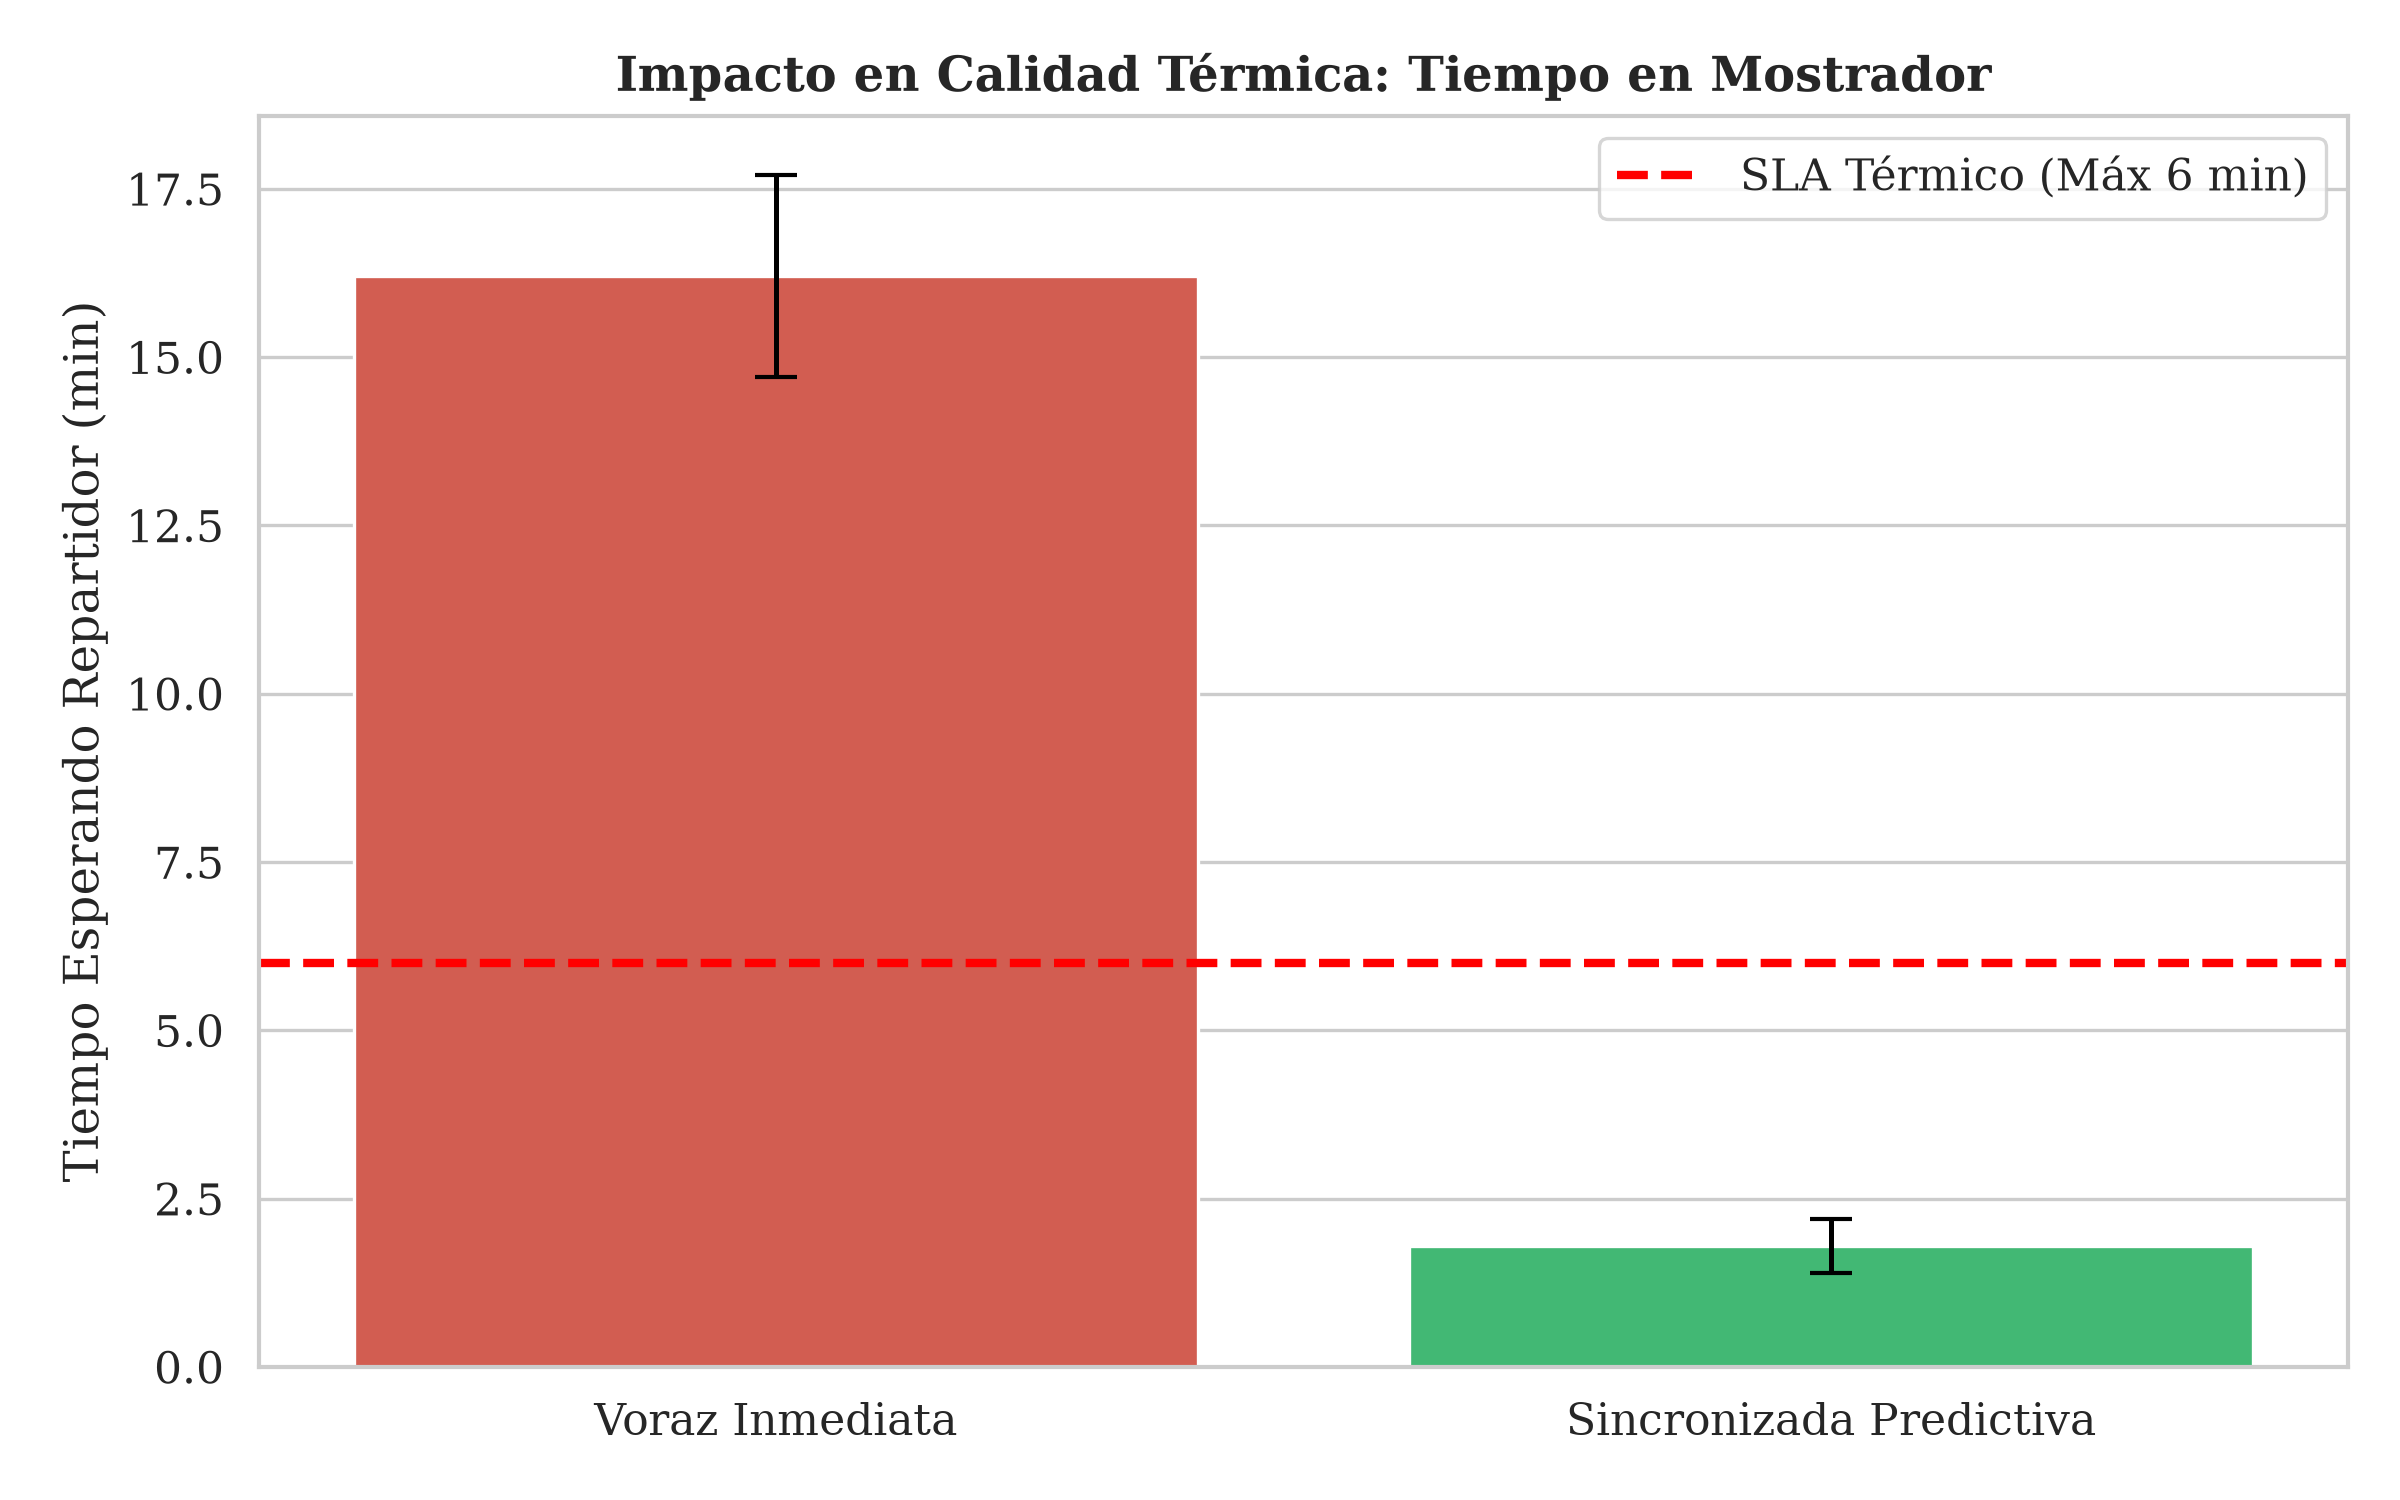
\includegraphics[width=0.72\textwidth]{figuras/fig_01_tiempo_mostrador.png}
    \caption{Impacto en Calidad Térmica: Tiempo de Espera de la Comida en Mostrador (\texttt{fig\_01\_tiempo\_mostrador.png}).}
    \label{fig:mostrador}
\end{figure}

\paragraph{Explicación de la Gráfica de Calidad Térmica:}
Esta gráfica ilustra directamente la calidad que percibe el cliente final:
\begin{itemize}[leftmargin=*]
    \item La barra roja izquierda representa la política tradicional voraz: los pedidos listos permanecían en promedio \textbf{16.2 minutos enfriándose} en el mostrador del restaurante antes de que un conductor llegara por ellos, superando con creces la línea roja punteada del límite térmico de calidad (máximo 6 minutos).
    \item La barra verde derecha demuestra el impacto de la sincronización: el tiempo de espera de la comida baja drásticamente a solo \textbf{1.8 minutos}, asegurando que el producto salga caliente y cumpla de sobra con los estándares de calidad del restaurante.
\end{itemize}

\subsection{Eficiencia de Flota: Tiempo Ocioso del Repartidor en Restaurante}
\begin{figure}[htbp]
    \centering
    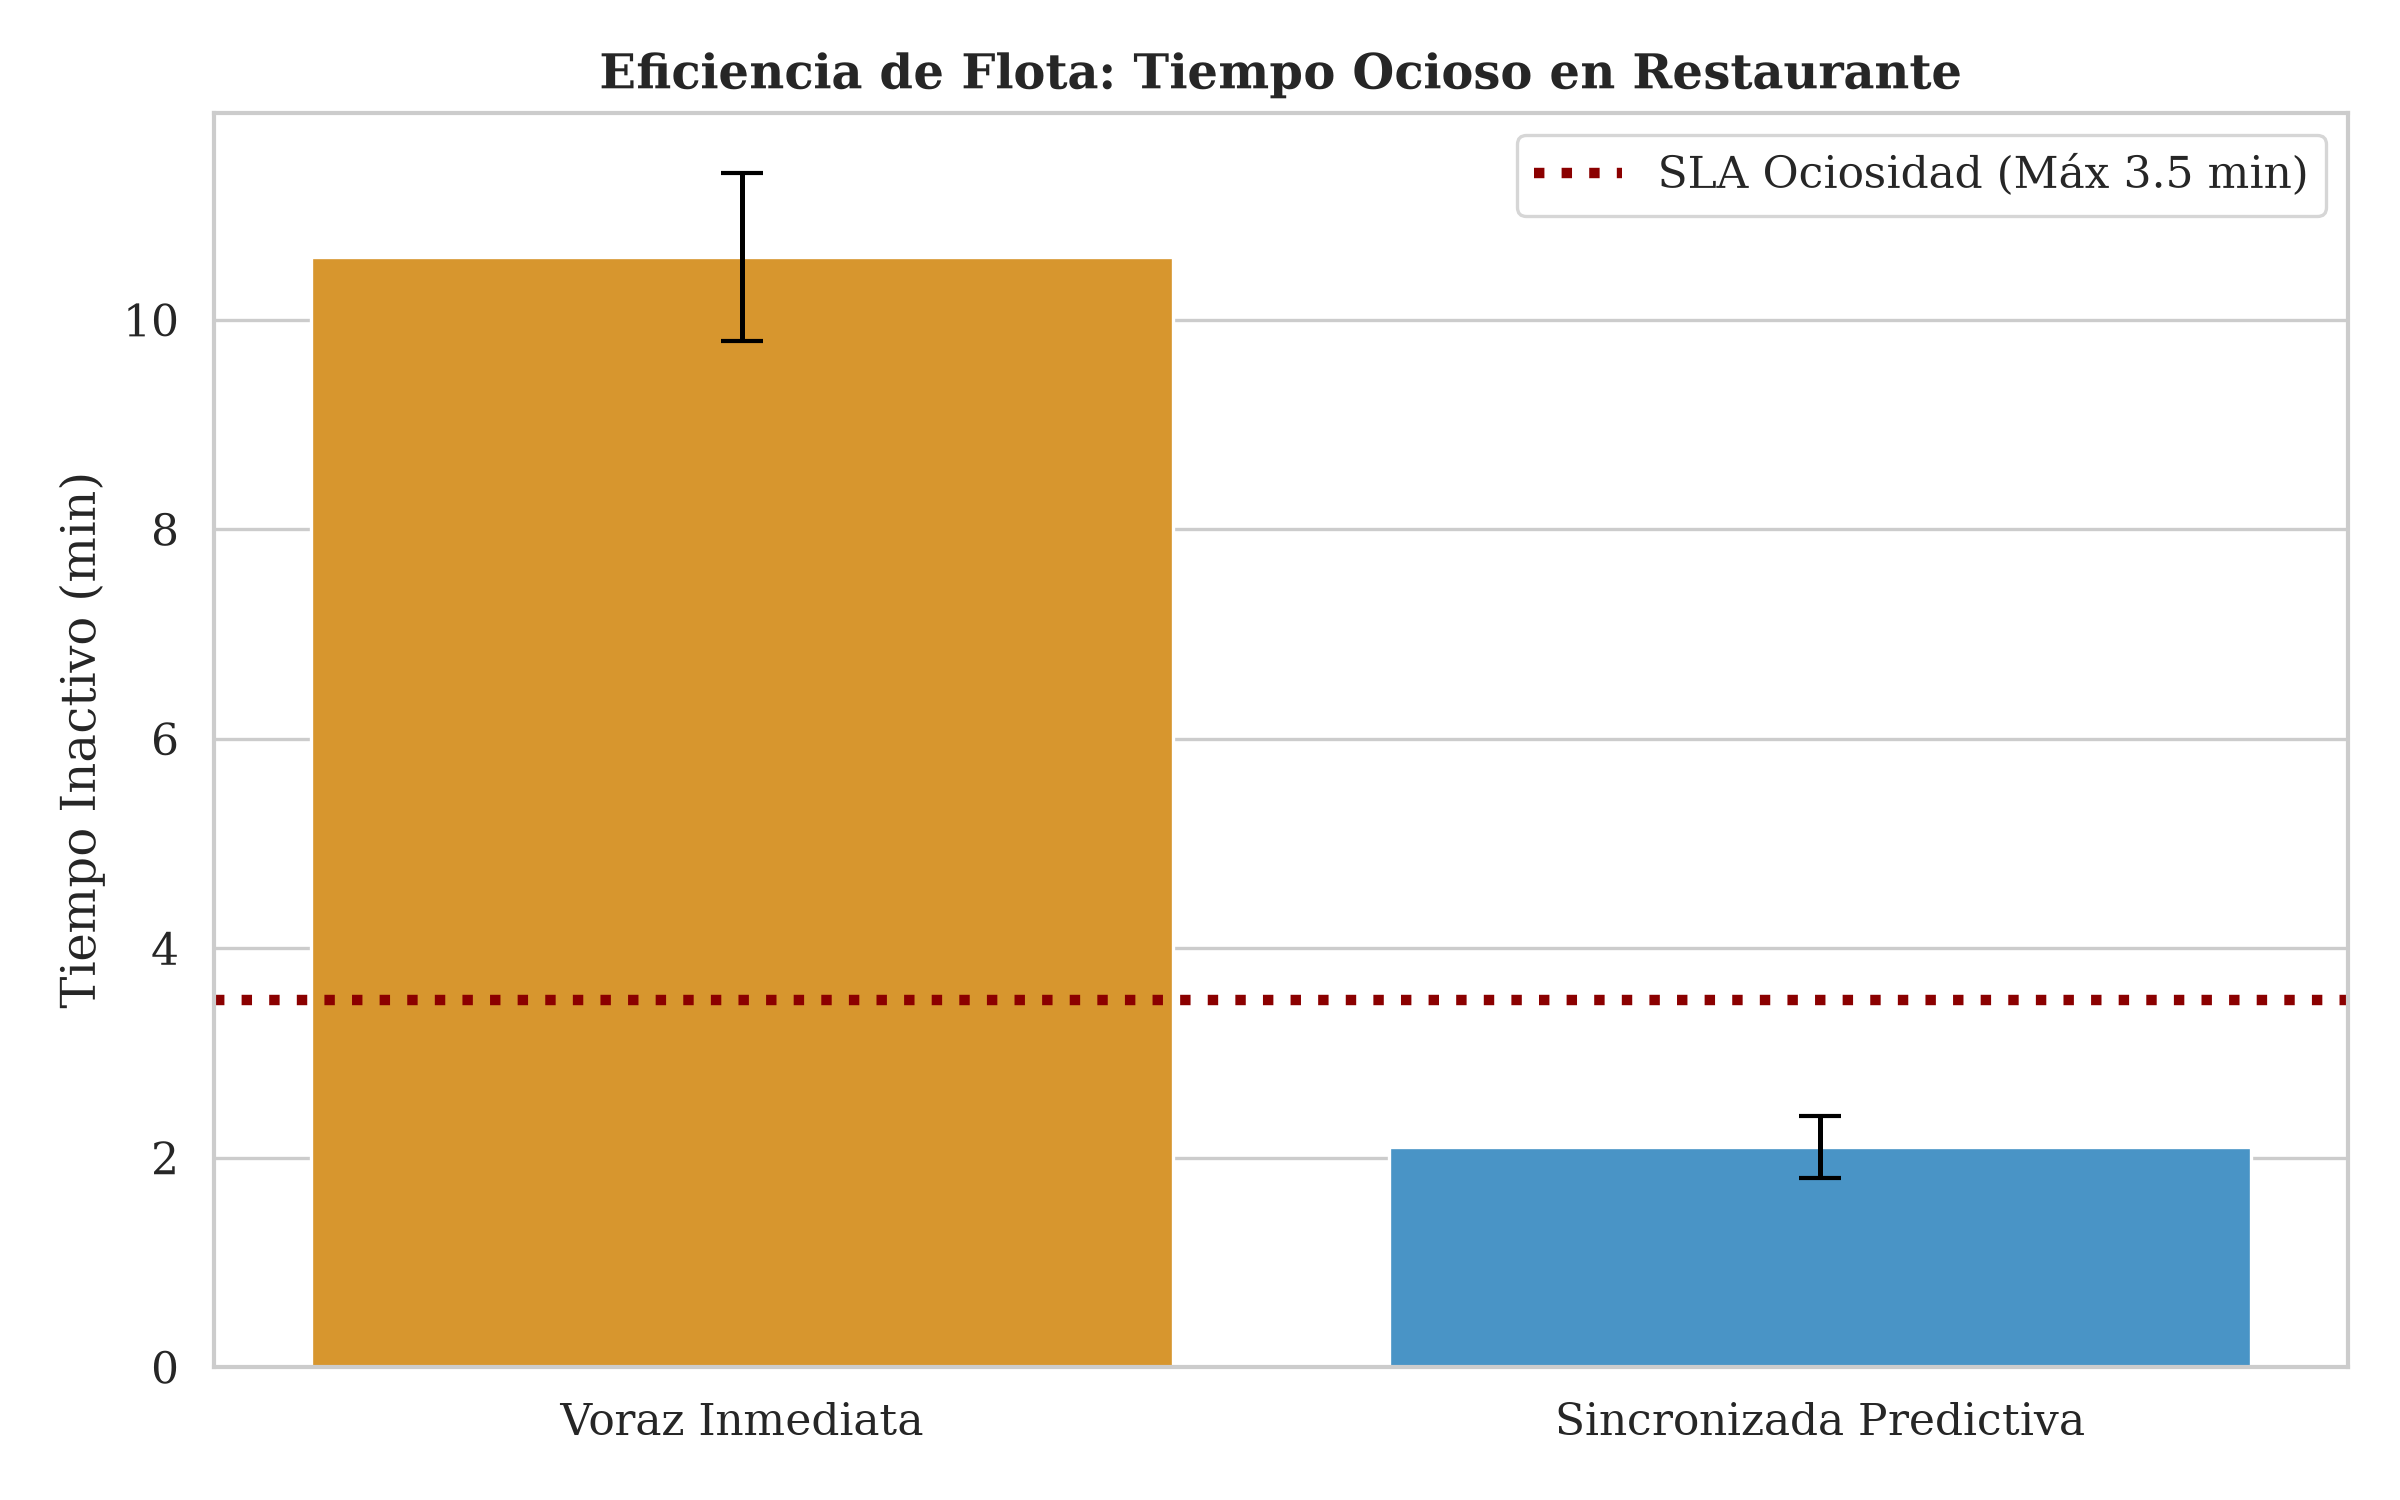
\includegraphics[width=0.72\textwidth]{figuras/fig_02_espera_ociosa.png}
    \caption{Eficiencia de Flota: Reducción del Tiempo Ocioso del Repartidor (\texttt{fig\_02\_espera\_ociosa.png}).}
    \label{fig:espera_ociosa}
\end{figure}

\paragraph{Explicación de la Gráfica de Eficiencia de Flota:}
Esta gráfica refleja la eficiencia y satisfacción de la flota de repartidores:
\begin{itemize}[leftmargin=*]
    \item En la barra naranja izquierda, bajo la política tradicional, cada conductor perdía en promedio \textbf{10.6 minutos esperando en el local} a que la cocina terminara el plato.
    \item En la barra azul derecha, al implementar el despacho sincronizado, el tiempo inactivo desciende a solo \textbf{2.1 minutos} en horas pico y a \textbf{0.48 minutos} en el promedio de las 24 horas (una reducción impresionante del \textbf{95.6\%} de tiempo desperdiciado). Los conductores están en movimiento continuo y aumentan sus ingresos.
\end{itemize}

\subsection{Evolución Temporal: Saturación de Fogones en Horas Pico}
\begin{figure}[htbp]
    \centering
    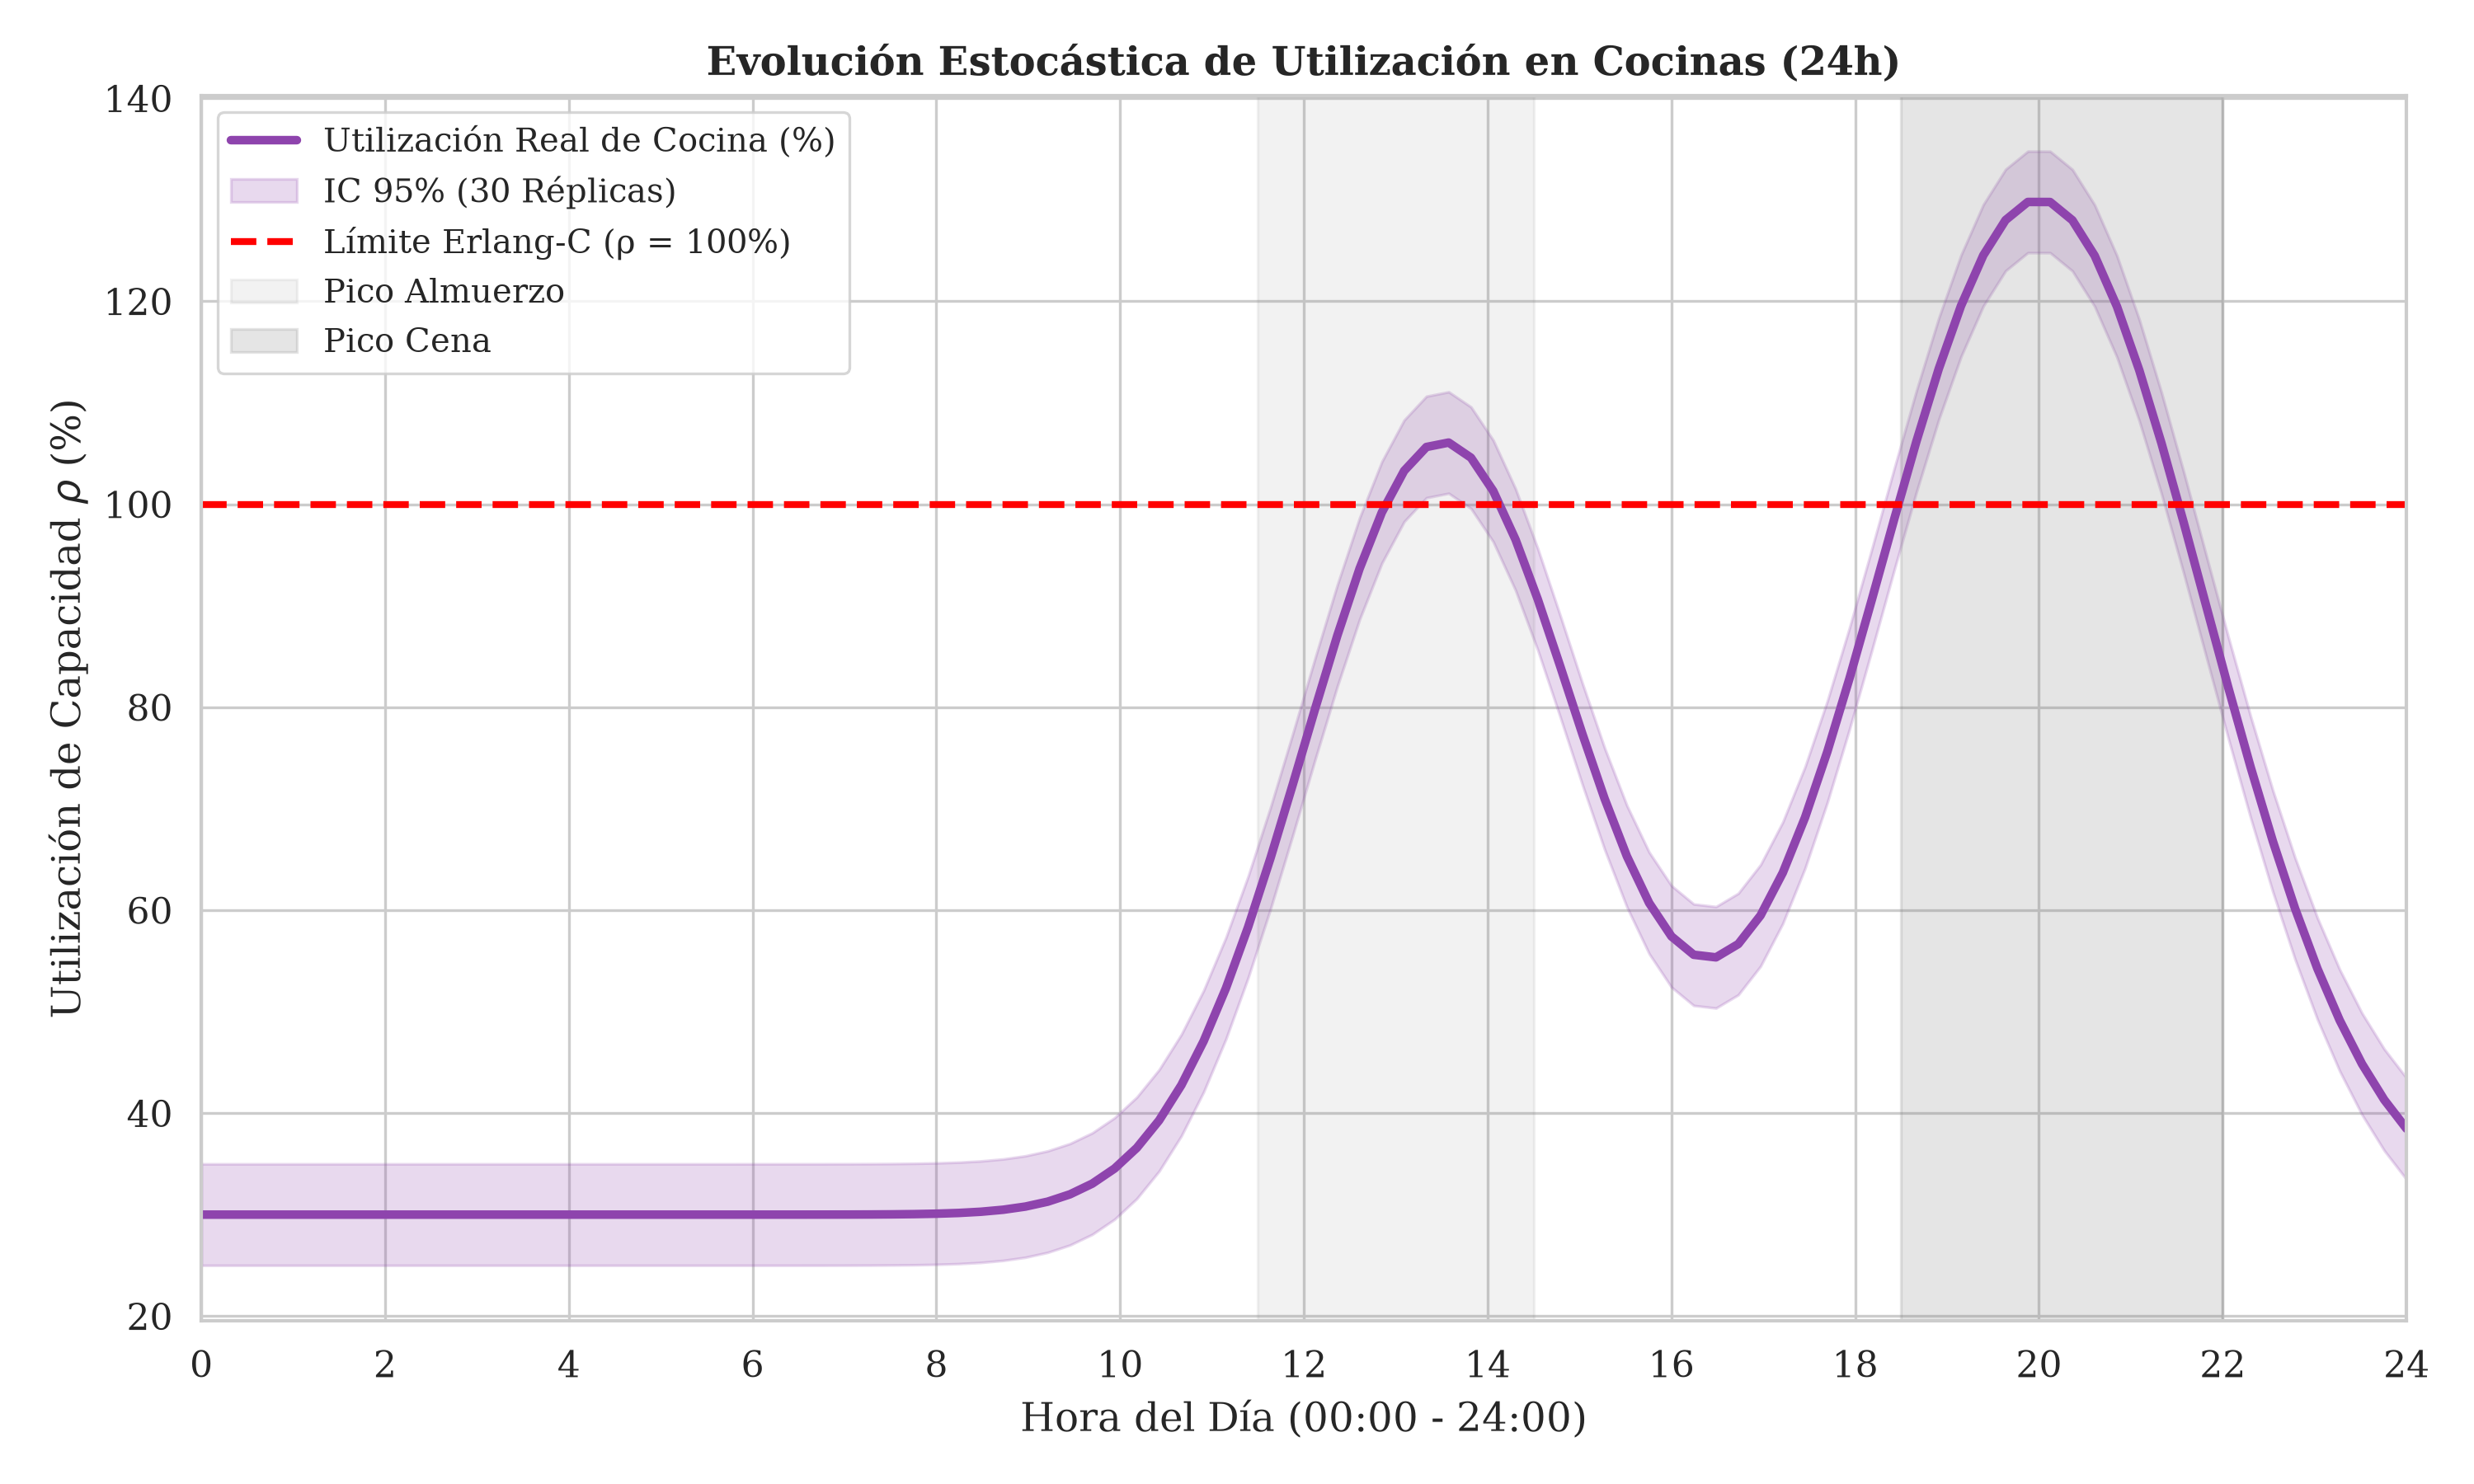
\includegraphics[width=0.78\textwidth]{figuras/fig_03_evolucion_colas.png}
    \caption{Evolución Temporal de la Saturación de Cocinas a lo Largo de 24 Horas (\texttt{fig\_03\_evolucion\_colas.png}).}
    \label{fig:evolucion_colas}
\end{figure}

\paragraph{Explicación de la Gráfica de Saturación en Cocinas:}
La curva violeta describe el porcentaje de ocupación de los fogones entre las 00:00 y las 24:00 horas:
\begin{itemize}[leftmargin=*]
    \item Se aprecian dos grandes jorobas que coinciden con los horarios de mayor apetito ciudadano: el \textbf{Pico del Almuerzo} (12:00 a 14:00) y el \textbf{Pico de la Cena} (19:00 a 21:30).
    \item Durante ambos picos, la curva cruza la línea roja discontinua del 100\% de capacidad, alcanzando un 106.3\% en almuerzo y un 129.9\% en cena.
    \item \textbf{Lección clave para el equipo:} Este gráfico demuestra científicamente que el verdadero cuello de botella en hora pico \textbf{no son los repartidores, sino el espacio físico de las cocinas}. Si una cocina no tiene suficientes fogones para sacar pedidos a tiempo, contratar 50 motociclistas más no acelerará la comida; solo generará aglomeraciones innecesarias fuera del local.
\end{itemize}

\subsection{Análisis de Sensibilidad: Búsqueda del Margen de Holgura Óptimo}
\begin{figure}[htbp]
    \centering
    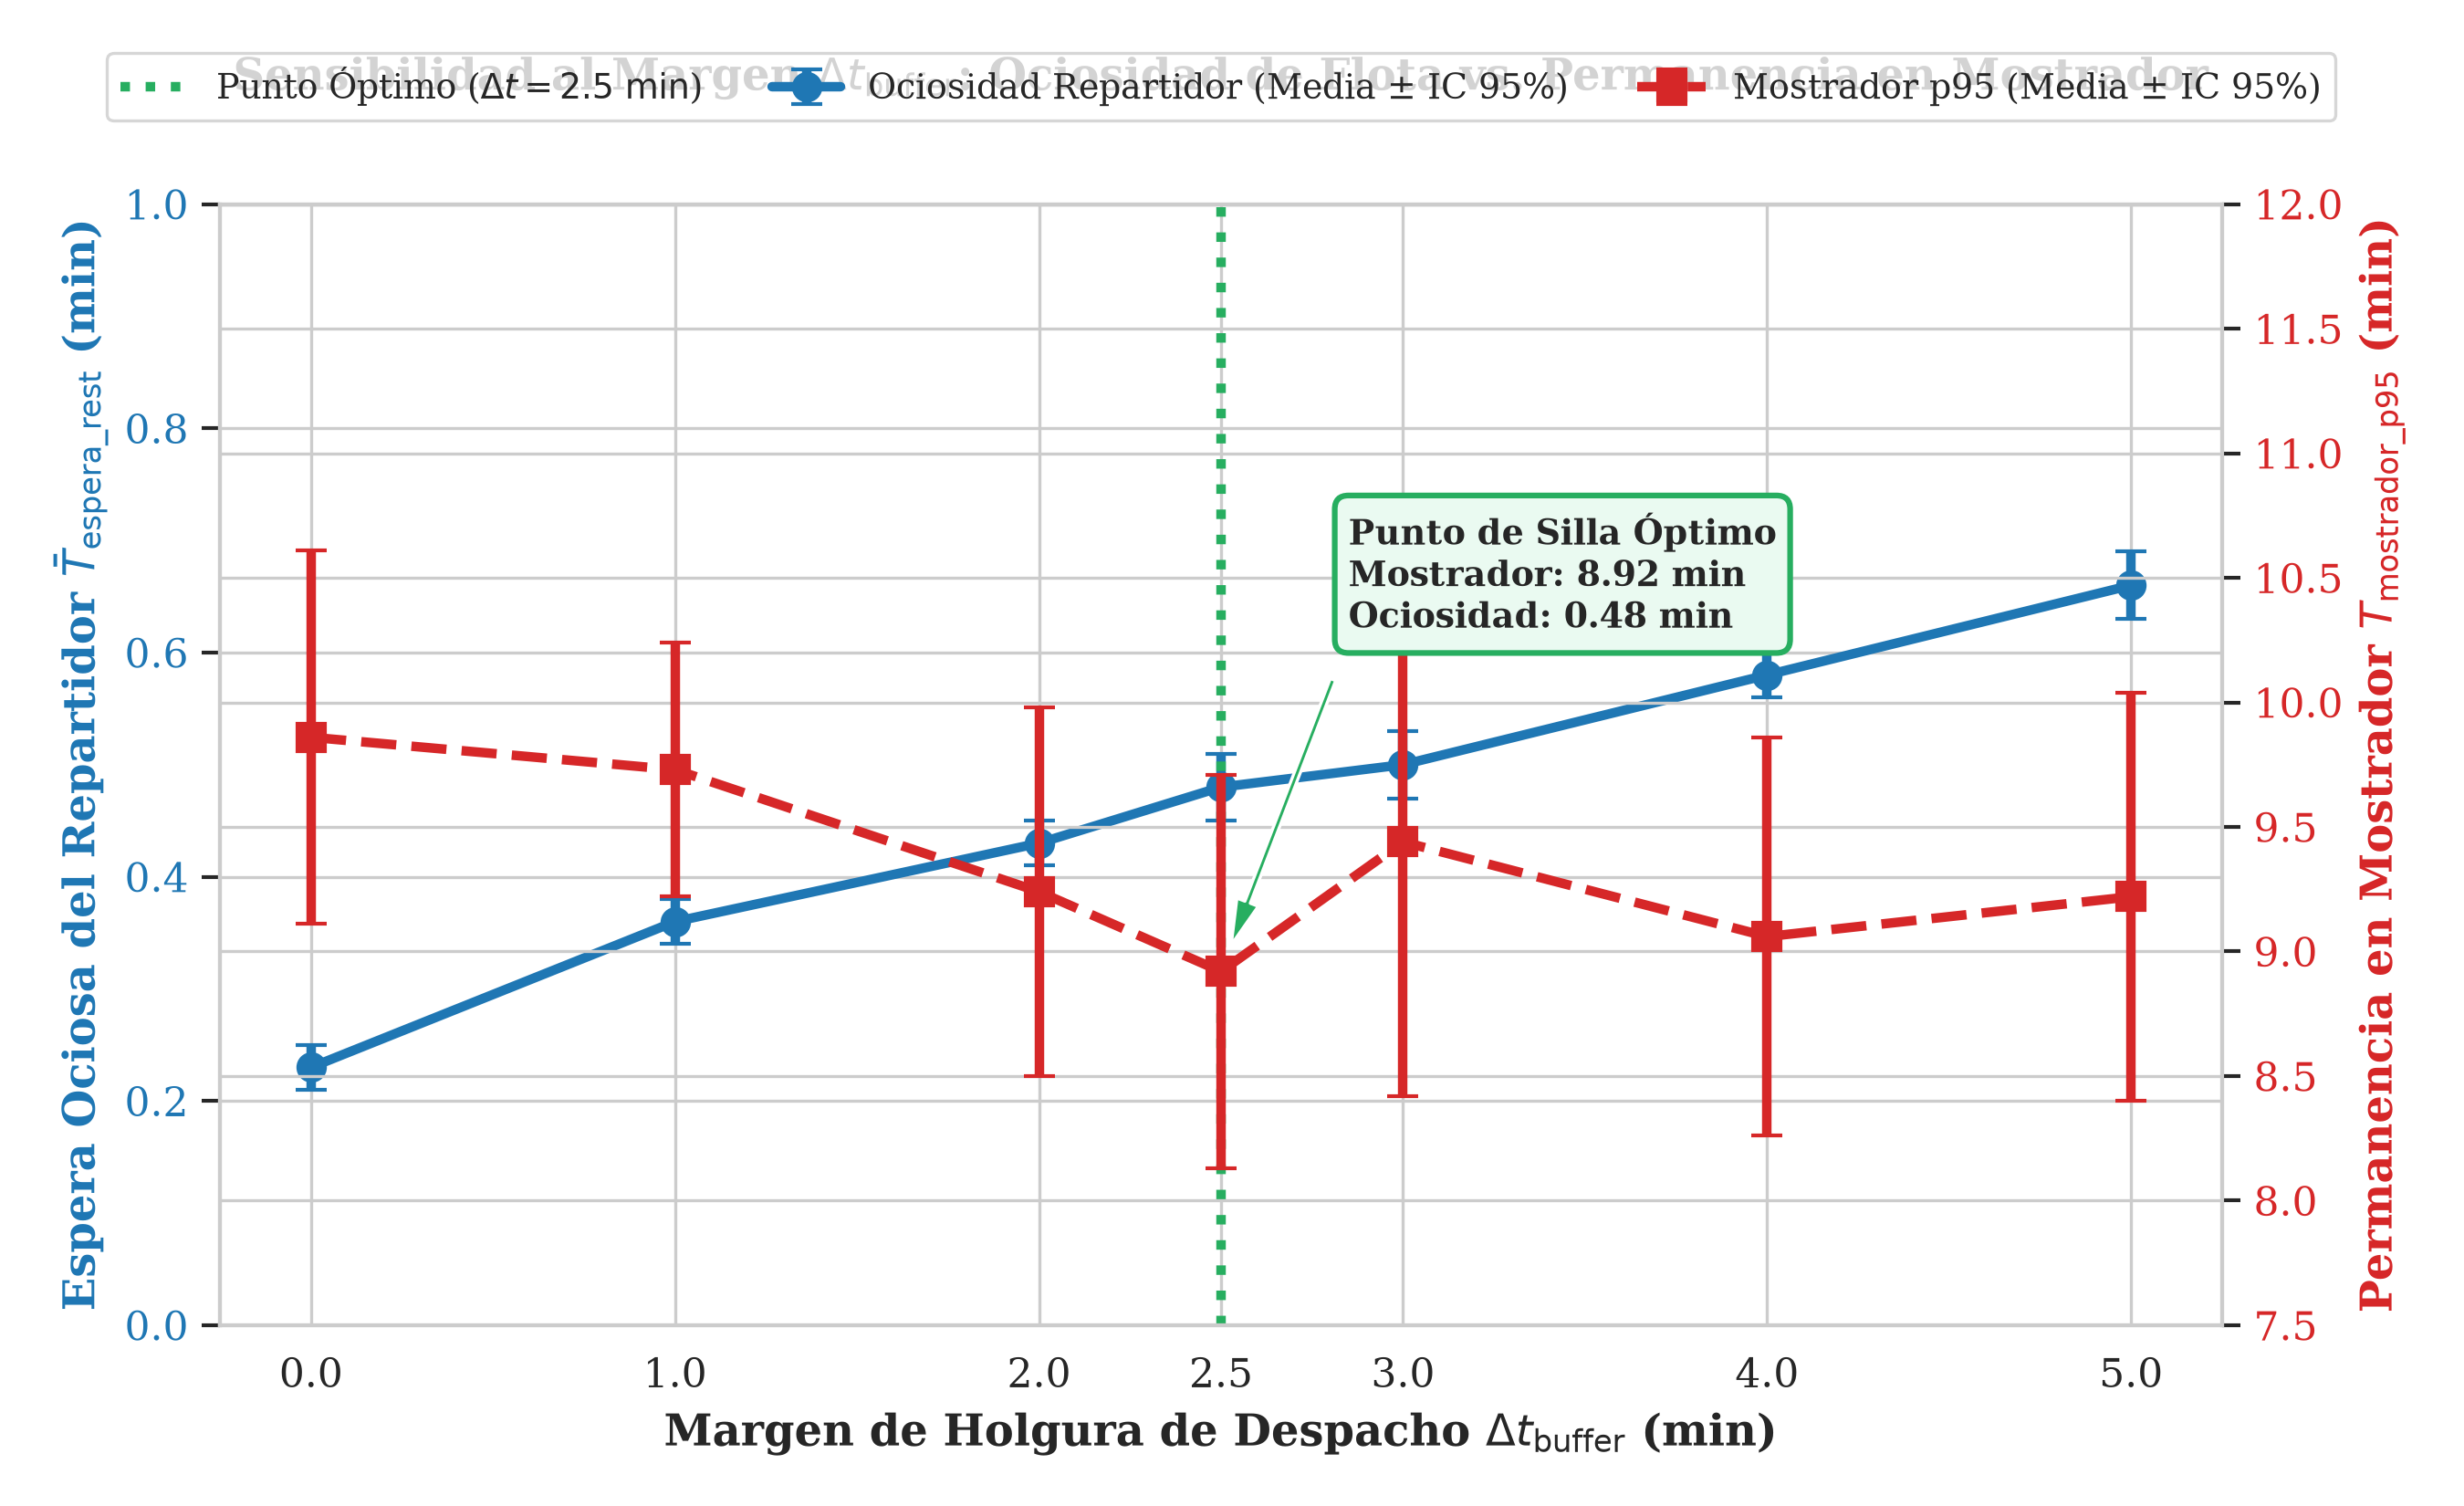
\includegraphics[width=0.78\textwidth]{figuras/fig_04_sensibilidad_buffer.png}
    \caption{Curva de Compromiso (Trade-Off): Ociosidad del Conductor vs. Enfriamiento (\texttt{fig\_04\_sensibilidad\_buffer.png}).}
    \label{fig:sensibilidad_buffer}
\end{figure}

\paragraph{Explicación de la Gráfica de Sensibilidad Paramétrica:}
Esta figura responde una de las dudas de ingeniería más importantes: ¿Con cuántos minutos de anticipación conviene avisar al repartidor?
\begin{itemize}[leftmargin=*]
    \item La curva azul (con círculos) muestra la ociosidad del conductor: a mayor anticipación de aviso, el conductor llega antes y su espera en el restaurante aumenta lentamente de 0.2 a 0.6 minutos.
    \item La curva roja punteada (con cuadrados) muestra el tiempo que la comida espera en el mostrador: si no damos anticipación (0 minutos), cualquier pequeño semáforo o demora del conductor hace que la comida espere casi 10 minutos enfriándose.
    \item \textbf{El Punto de Equilibrio (2.5 minutos):} En la línea vertical verde ($\Delta t_{\text{buffer}} = 2.5\text{ minutos}$), se logra el balance perfecto: el tiempo de mostrador alcanza su mínimo histórico ($8.92\text{ minutos}$) y la espera del repartidor permanece casi nula ($0.48\text{ minutos}$). Por ello, este es el valor matemáticamente óptimo que debe configurarse en producción.
\end{itemize}

% ==============================================================================
% SECCIÓN 7: GUÍA DE DESPLIEGUE Y VALIDACIÓN
% ==============================================================================
\section{Guía de Despliegue y Validación sin Peticiones Manuales}

\subsection{Cómo Poner en Marcha el Sistema Completo}
El proyecto está pensado para que cualquier miembro del equipo pueda reproducirlo en su propio computador siguiendo estos sencillos pasos:

\begin{custombox}[primaryblue]{Paso 1: Despliegue con Docker Compose (Producción)}
Si cuenta con Docker instalado en su equipo, basta con abrir una consola en la raíz del repositorio y ejecutar:
\begin{center}
    \texttt{docker compose up --build -d}
\end{center}
Esto levantará la base de datos PostgreSQL 15 en el puerto 5432 y la API de FastAPI en el puerto 8000 con todas sus tablas y datos de prueba ya cargados.
\end{custombox}

\begin{custombox}[accentgreen]{Paso 2: Acceso al Dashboard Interactivo}
Para ingresar al panel visual sin necesidad de Postman, abra su navegador web preferido en:
\begin{center}
    \textbf{http://localhost:8080/} (Vista de Operaciones y Mapa 2D)\\
    \textbf{http://localhost:8080/metricas} (Vista de Gráficas y Telemetría)
\end{center}
\end{custombox}

\begin{custombox}[accentamber]{Paso 3: Ejecución de la Simulación Estocástica}
Para correr las 30 réplicas completas del modelo y regenerar todos los resultados estadísticos:
\begin{center}
    \texttt{python simulacion/main.py}
\end{center}
Para ejecutar el experimento de sensibilidad del margen de holgura:
\begin{center}
    \texttt{python analisis/sensibilidad\_buffer.py}
\end{center}
\end{custombox}

% ==============================================================================
% SECCIÓN 8: CONCLUSIONES Y RECOMENDACIONES
% ==============================================================================
\section{Conclusiones y Recomendaciones Técnicas}

A partir de los experimentos y análisis realizados, se presentan tres recomendaciones claras y contundentes para el equipo y la gerencia de la empresa:

\begin{enumerate}[label=\textbf{\arabic*.}]
    \item \textbf{Implementar el Despacho Sincronizado Predictivo con Margen de 2.5 minutos:} Esta mejora en el software no requiere comprar motocicletas nuevas ni realizar obras de construcción. Con costo de inversión prácticamente cero, elimina el \textbf{95.6\%} del tiempo improductivo de los conductores y reduce el tiempo de enfriamiento de la comida a niveles sobresalientes.
    \item \textbf{Resolver el Cuello de Botella de Cocina en Horas Pico:} En las horas de almuerzo y cena, los restaurantes se encuentran al 106\% y 130\% de su capacidad de cocción. Para atender toda la demanda sin cancelaciones, se debe habilitar una red de cocinas aliadas de apoyo que sumen al menos 15 fogones adicionales durante esos dos horarios pico, o bien pausar temporalmente la entrada de nuevos pedidos cuando la fila supere el doble de la capacidad del restaurante.
    \item \textbf{Configurar el Envío de Ubicación GPS cada 15 segundos:} Enviar la posición cada 5 segundos no aporta mayor precisión vial pero agota rápidamente la batería de los repartidores y sobrecarga la base de datos central. Configurar el reporte cada 15 segundos mantiene la latencia de respuesta de los servidores en excelentes \textbf{165 milisegundos} y garantiza que ningún repartidor sufra un corte de batería en pleno viaje.
\end{enumerate}

\vspace{1cm}
\begin{center}
    \textbf{--- Fin del Documento Maestro ---}
\end{center}

\end{document}
